\documentclass[11pt]{article}

\usepackage[margin=1in]{geometry}
\usepackage[T1]{fontenc}
\usepackage[utf8]{inputenc}
\usepackage{lmodern}
\usepackage{microtype}
\usepackage{amsmath,amssymb,mathtools}
\usepackage{hyperref}
\usepackage{graphicx}
\usepackage{subcaption}
\usepackage{float}
\hypersetup{hidelinks}

\title{Meeting notes on preconditioned operator GD on $S^1$}
\author{Shreyas Kalvankar}
\date{\today}

\begin{document}
\maketitle

\section*{Summary}

We study how well a Fourier-block preconditioner works for a high-frequency target.

We use the target
\begin{align*}
	f^*(\gamma)
	 & =
	1
	+0.9\cos(\gamma)
	+0.5\cos(2\gamma)
	-0.35\sin(3\gamma) \\
	 & \quad
	+0.25\cos(7\gamma)
	-0.10\sin(10\gamma)
	+0.08\cos(12\gamma)
	-0.04\sin(15\gamma),
\end{align*}
and compare three settings:

\begin{enumerate}
	\item \textbf{Small preconditioning block:} $K_{\max}=8$, so modes $10,12,15$ lie outside the block.

	\item \textbf{Out-of-block modes removed:} same block $K_{\max}=8$, but the target is restricted to
	      \[
		      f^*(\gamma)
		      =
		      1
		      +0.9\cos(\gamma)
		      +0.5\cos(2\gamma)
		      -0.35\sin(3\gamma)
		      +0.25\cos(7\gamma).
	      \]

	\item \textbf{Full block:} $K_{\max}=16$, so all target modes are included in the preconditioner.
\end{enumerate}

Main observations:
\begin{itemize}
	\item If all active modes lie inside the block, preconditioning makes their decay rates similar.
	\item If some active modes lie outside the block, preconditioning still helps, but cannot remove their effect completely.
	\item The empirical preconditioner is closest to ideal. The theory version improves as the sample size increases.
\end{itemize}

\section*{1. Setup}

We parameterize the circle by $\gamma\in[0,2\pi)$ and embed it as
\[
	x(\gamma)=(\cos\gamma,\sin\gamma).
\]
For each run, we sample training angles
\[
	\gamma_1,\dots,\gamma_n \overset{\mathrm{iid}}{\sim} \mathrm{Unif}[0,2\pi),
\]
form the analytic kernel matrix
\[
	K_{ij}=\Theta(\gamma_i,\gamma_j),
\]
and define the normalized empirical operator
\[
	A=\frac{1}{n}K.
\]

To study low-frequency structure, we evaluate the real Fourier basis up to some cutoff $K_{\max}$:
\[
	\phi_0(\gamma)=1,
\]
\[
	\phi_{k,c}(\gamma)=\sqrt{2}\cos(k\gamma),\qquad
	\phi_{k,s}(\gamma)=\sqrt{2}\sin(k\gamma),
	\qquad k=1,\dots,K_{\max}.
\]
This gives the sampled basis matrix
\[
	\Phi\in\mathbb{R}^{n\times d},
	\qquad d=2K_{\max}+1.
\]

The associated sampled block objects are
\[
	G=\frac{1}{n}\Phi^\top\Phi,
	\qquad
	H=\frac{1}{n}\Phi^\top A\Phi,
	\qquad
	C=G^{-1}H.
\]
Here $C$ is the effective empirical operator on the retained Fourier block.

We also use the finite-$n$ eigenvalues
\[
	\Lambda^{(n)}=\mathrm{diag}(\lambda_p^{(n)}),
	\qquad
	\lambda_p^{(n)}=
	\left(1-\frac1n\right)\lambda_{k_p}+\frac1n g(0),
\]
where $g(0)=\Theta(x,x)$.

\section*{2. The three flows}

We compare three residual flows:
\[
	\dot r=-\eta B r,
	\qquad r(t)=y(t)-y^*.
\]

\paragraph{Baseline.}
\[
	B=A.
\]

\paragraph{Theory-preconditioned flow.}
\[
	P_{\mathrm{th}}=\frac1n \Phi (\Lambda^{(n)})^{-1} G^{-1}\Phi^\top,
	\qquad
	B_{\mathrm{th}}=P_{\mathrm{th}}A.
\]

\paragraph{Empirical-preconditioned flow.}
\[
	P_{\mathrm{emp}}=\frac1n \Phi C^{-1} G^{-1}\Phi^\top,
	\qquad
	B_{\mathrm{emp}}=P_{\mathrm{emp}}A.
\]

The point of both preconditioners is the same: we do not try to invert the full empirical operator. We only try to correct the dynamics on the retained Fourier block.

\section*{3. Why the residual curves do not all decay to the same final level}

At first sight, if the preconditioned block operator is close to identity, one might expect every retained mode to decay to zero at the same rate. In practice, this is not what we observe: the curves drop quickly and then level off at different small values.

The reason is that the sampled Fourier modes are only approximate eigenvectors.

In the ideal case, we would have
\[
	A\Phi=\Phi\Lambda^{(n)}.
\]
In reality,
\[
	A\Phi=\Phi\Lambda^{(n)}+E,
\]
where
\[
	E:=A\Phi-\Phi\Lambda^{(n)}
\]
is the finite-sample action error.

Because of this error, the modes are not perfectly decoupled, and there is always some leakage between the retained Fourier coordinates and the rest of sample space.

To understand the effect on a single mode, consider the ideal case where the modes are exact eigenvectors:
\[
	\dot \alpha_p = -\eta \lambda_p \alpha_p.
\]
Each mode then decays independently.

In practice, a simple model is
\[
	\dot \alpha_p = -\eta \lambda_p^{(n)} \alpha_p + \text{leakage}_p(t),
\]
where the leakage term represents coupling from other modes and from components outside the retained block.

At steady state, decay and leakage balance:
\[
	\eta \lambda_p^{(n)} \alpha_p \approx \text{leakage level},
	\qquad
	\Rightarrow
	\qquad
	\alpha_p \approx \frac{\text{leakage}_p}{\eta \lambda_p^{(n)}}.
\]

This explains the different floors. Modes with smaller eigenvalues suppress leakage less effectively and therefore stop at higher residual levels, while modes with larger eigenvalues decay further.

This effect is most visible when the target contains modes outside the preconditioning block. In that case, the leakage term remains nonzero and acts as a persistent source. If all active modes are included in the preconditioning block, this leakage is much smaller, and the final residual levels become more uniform across modes.

\section*{4. Experiments with high-frequency targets}

We now compare three settings using a high-frequency target. The difference between them is how the preconditioning block relates to the active target frequencies.

\subsection*{4.1 High-frequency target with a small preconditioning block}

In this setting, the target contains frequencies that lie outside the retained Fourier block used for preconditioning. So the preconditioner only acts on part of the signal.

\begin{figure}[H]
	\centering
	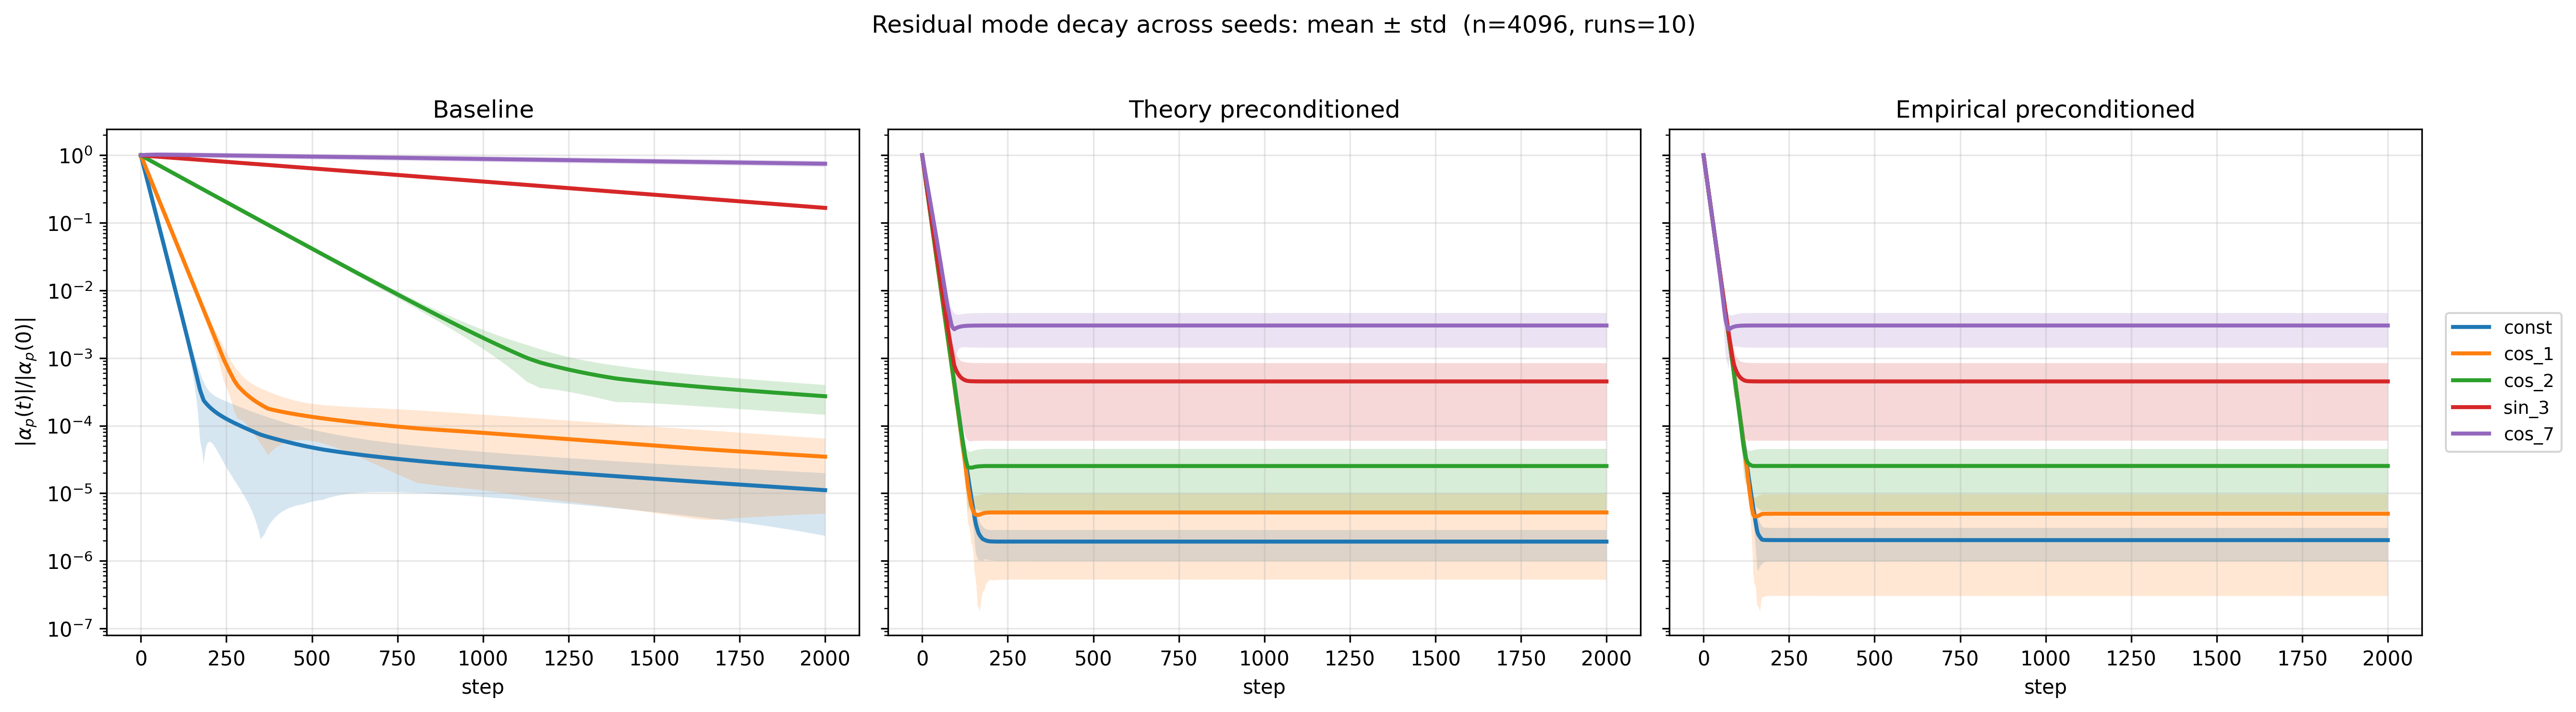
\includegraphics[width=\textwidth]{images/target-high-frequency-with-low-sample-block/all_mode_decay_three_panel_mean_std_n4096.png}
	\caption{High-frequency target with a small preconditioning block. The baseline shows strong separation across modes. Both preconditioned flows align the retained modes, but different modes settle at different residual levels.}
\end{figure}

This matches the discussion in Section 3. The modes outside the retained block act as a source of leakage. Since higher-frequency modes have smaller effective eigenvalues, they suppress this leakage less effectively and therefore stop at higher residual levels.

\subsection*{4.2 Same block, but out-of-block modes removed}

Here we use the same preconditioning block, but remove all target frequencies outside that block. So the target lies entirely inside the retained subspace.

\begin{figure}[H]
	\centering
	
\includegraphics[width=\textwidth]{images/target-high-frequency-with-low-sample-block-out-of-block-removed/all_mode_decay_three_panel_mean_std_n4096.png}
	\caption{Same preconditioning block, but with out-of-block target modes removed. The residual floors are much lower and more uniform across modes.}
\end{figure}

In this case, the leakage term is much smaller because there is no longer a persistent source coming from outside the block. As a result, all modes decay further and the differences between their final levels are reduced.

\subsection*{4.3 High-frequency target with full preconditioning block}

Finally, we increase the preconditioning block so that it includes all active target frequencies.

\begin{figure}[H]
	\centering
	
\includegraphics[width=\textwidth]{images/target-high-frequency-all-preconditioned/all_mode_decay_three_panel_mean_std_n4096.png}
	\caption{High-frequency target with all active modes included in the preconditioning block. The empirical preconditioner makes the decay almost identical across modes.}
\end{figure}

Now the preconditioner acts on all active modes. The effective eigenvalues are close to uniform, and the leakage is minimal. As a result, the residual curves align closely and decay to similar levels.

\paragraph{Theory vs empirical preconditioning.}

\begin{itemize}
	\item The theory preconditioner uses only the eigenvalues $\Lambda^{(n)}$.
	\item It assumes the Fourier basis diagonalizes the operator.
	\item The empirical preconditioner uses $C=G^{-1}H$.
	\item This captures both eigenvalues and small deviations in eigenvectors.
\end{itemize}

So:
\begin{itemize}
	\item Theory corrects scaling.
	\item Empirical corrects both scaling and alignment.
\end{itemize}

As $n$ increases:
\begin{itemize}
	\item The operator becomes closer to diagonal in the Fourier basis.
	\item The two preconditioners become closer.
\end{itemize}

\paragraph{Evidence from the block spectra.}

The difference between the two preconditioners is visible in the spectrum of the
compressed block.

\begin{figure}[H]
	\centering
	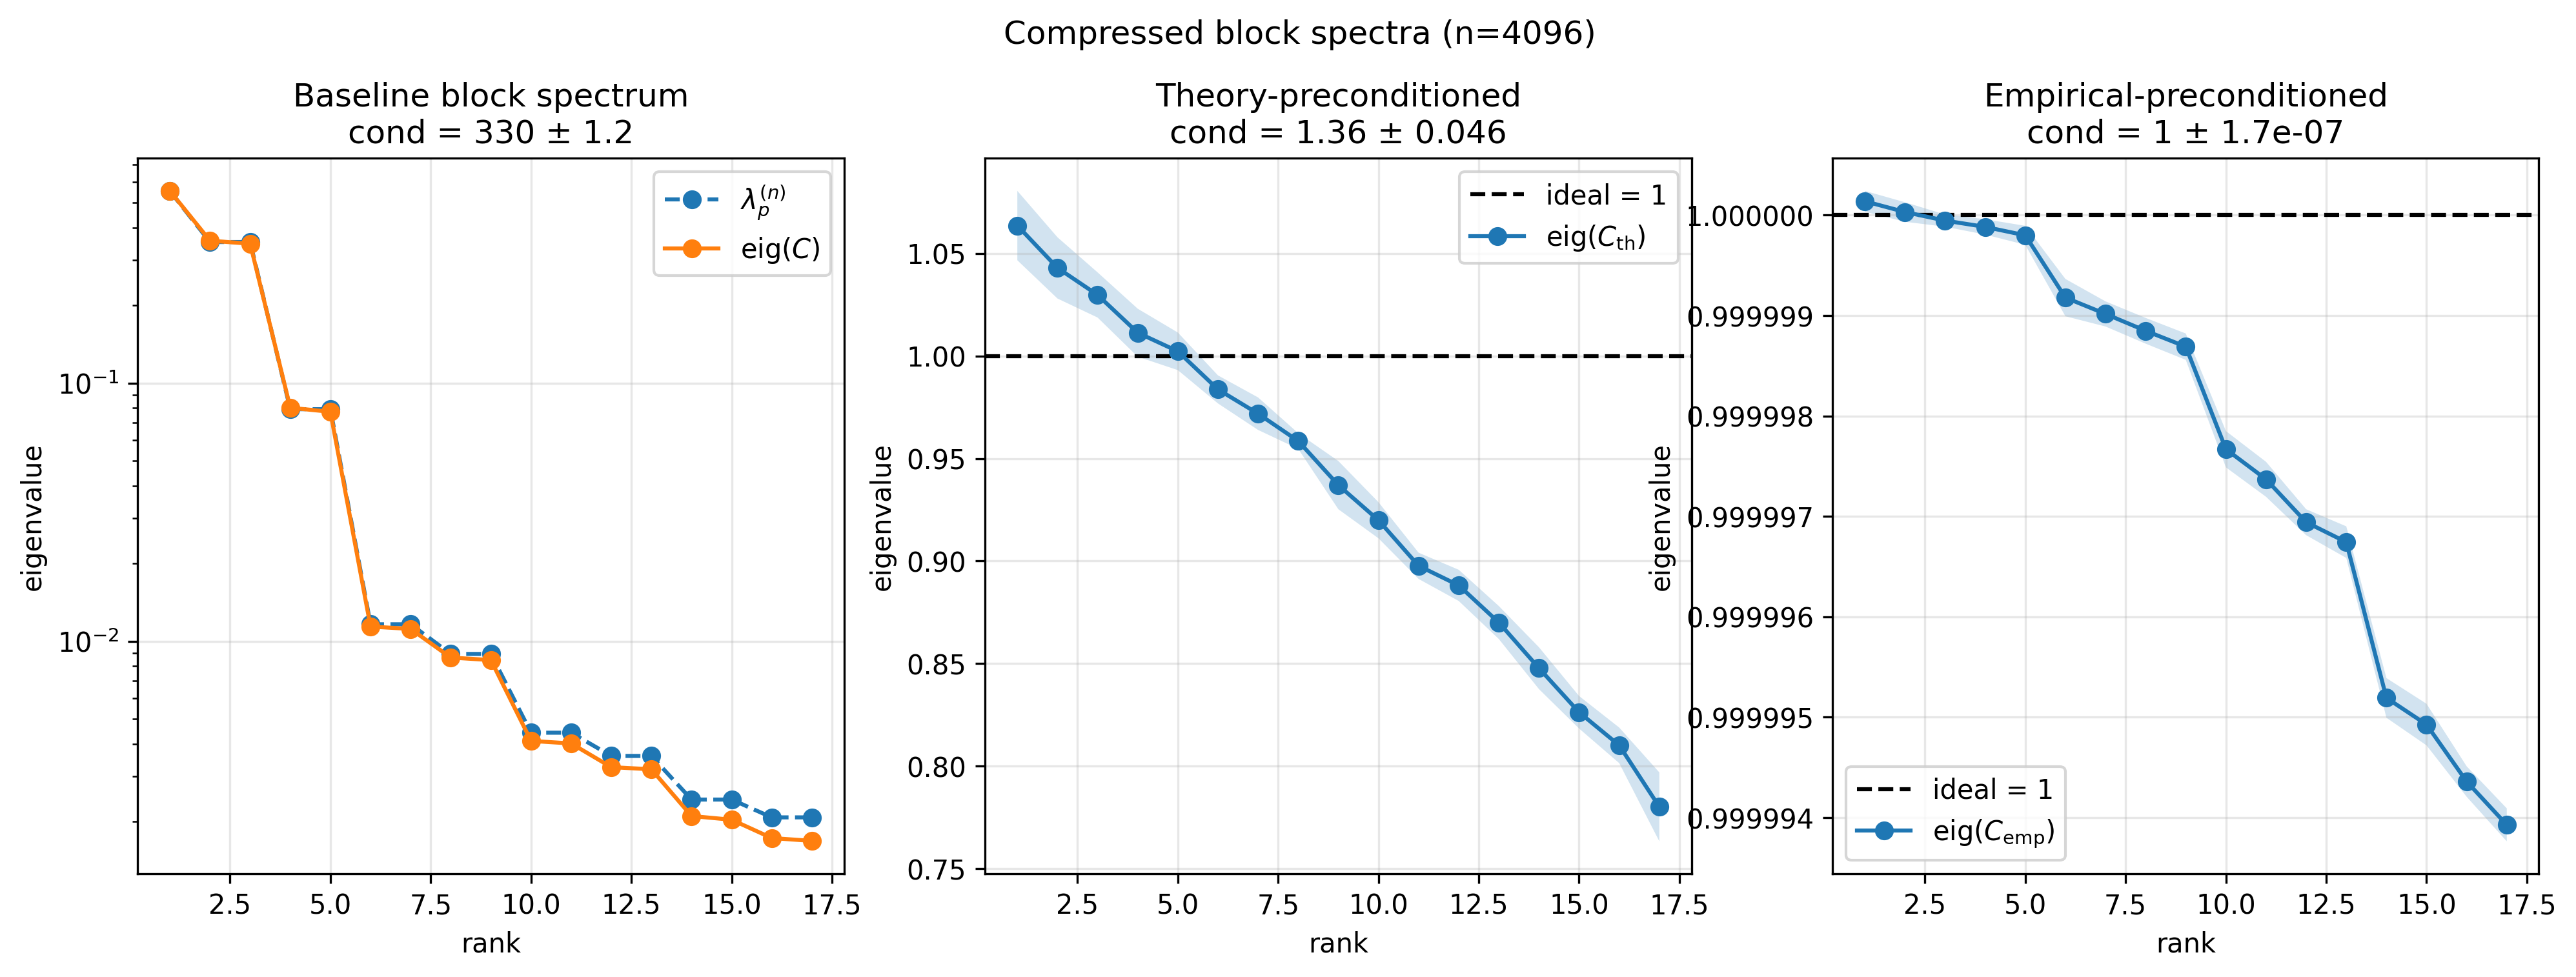
\includegraphics[width=\textwidth]{images/target-high-frequency-with-low-sample-block-out-of-block-removed/compressed_block_spectra_4096.png}
	\caption{Block spectrum at $n=4096$. Baseline has a wide spread. Theory preconditioning reduces the spread but leaves a slope. Empirical preconditioning is almost flat at $1$.}
	\label{fig:block-spectra-4096}
\end{figure}

\begin{figure}[H]
	\centering
	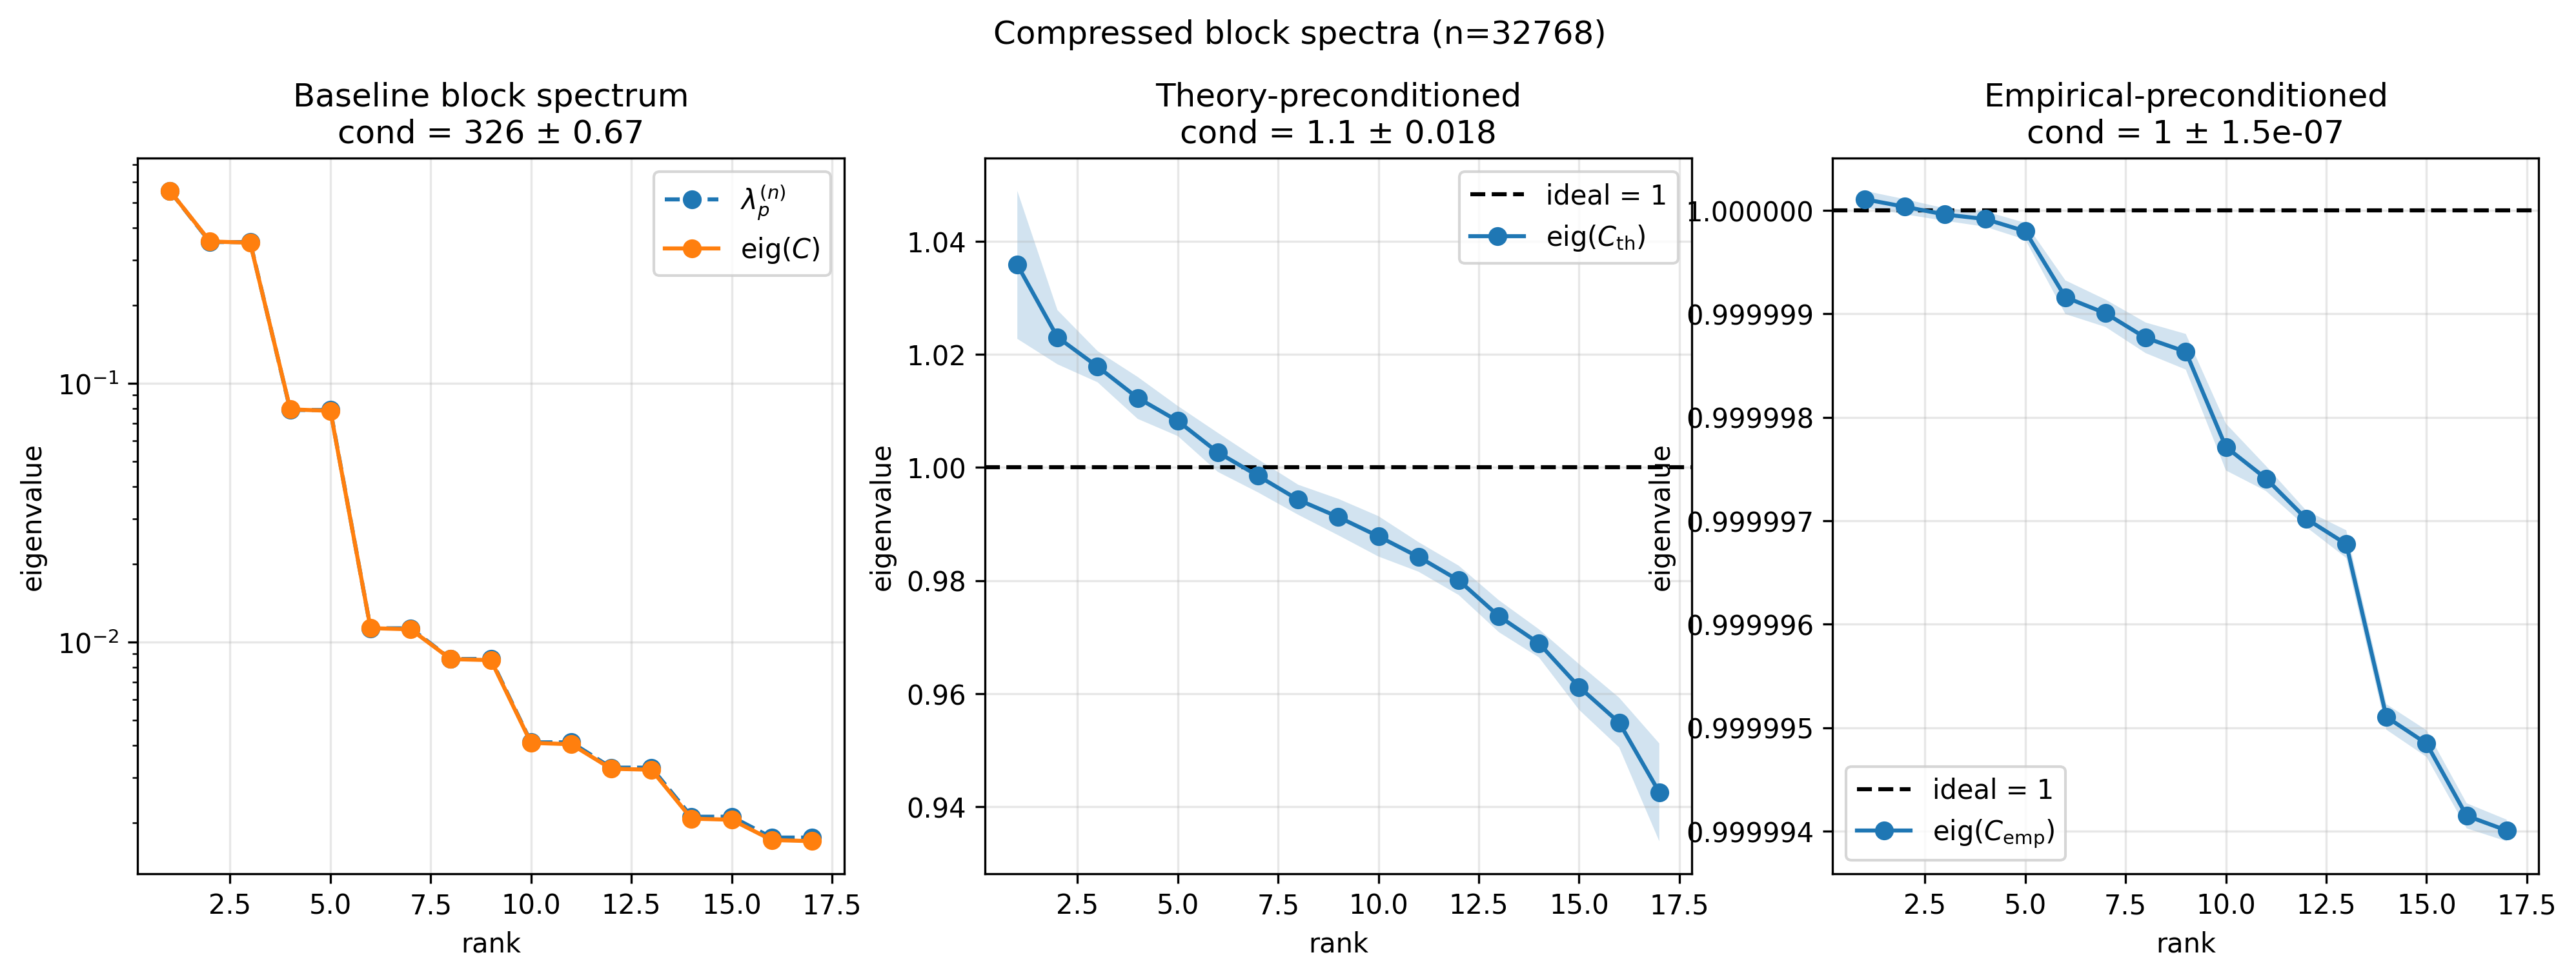
\includegraphics[width=\textwidth]{images/target-high-frequency-with-low-sample-block-out-of-block-removed/compressed_block_spectra_32768.png}
	\caption{Block spectrum at $n=32768$. The theory-preconditioned spectrum becomes flatter and closer to the empirical case.}
	\label{fig:block-spectra-32768}
\end{figure}

\begin{figure}[H]
	\centering
	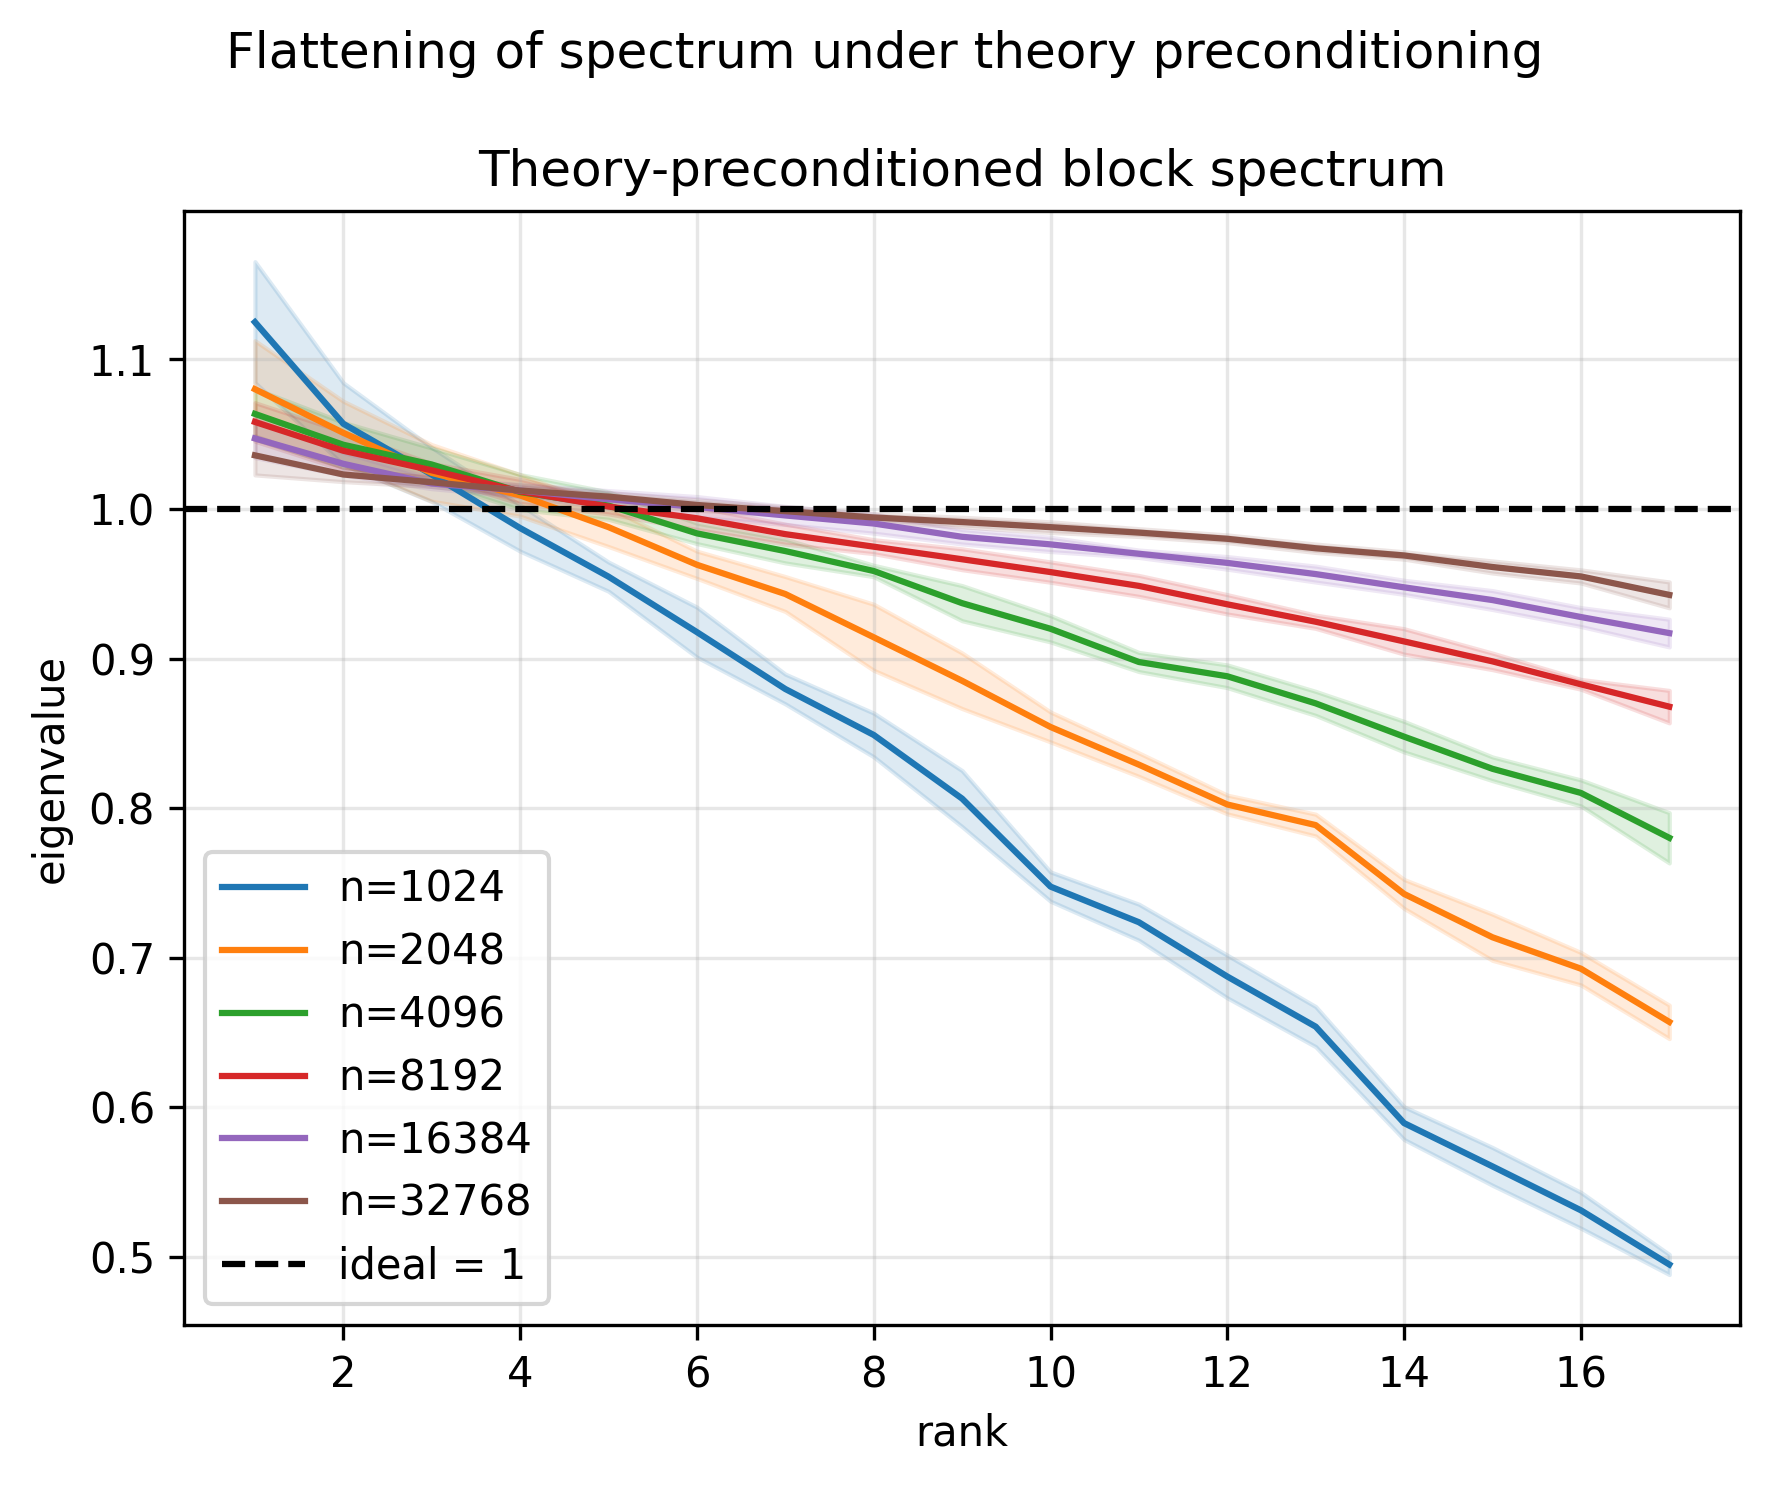
\includegraphics[width=0.75\textwidth]{images/target-high-frequency-with-low-sample-block-out-of-block-removed/theory_preconditioned_spectrum_all_n.png}
	\caption{Effect of increasing $n$. The theory-preconditioned spectrum approaches $1$ as $n$ increases.}
	\label{fig:block-spectra-all-n}
\end{figure}

Summary:
\begin{itemize}
	\item Baseline: wide spread of eigenvalues.
	\item Theory: flattens the spectrum but does not make it constant.
	\item Empirical: almost exactly flat at $1$.
	\item As $n$ increases, the theory curve moves closer to the empirical one.
\end{itemize}

\section*{5. Convergence with increasing sample size}

$P_{\mathrm{th}}$ and $P_{\mathrm{emp}}$ are the preconditioners, and
$B_{\mathrm{th}}$, $B_{\mathrm{emp}}$ are the operators used in the dynamics.

As $n$ increases:
\begin{itemize}
	\item $C$ gets closer to $\Lambda^{(n)}$,
	\item $P_{\mathrm{th}}$ gets closer to $P_{\mathrm{emp}}$,
	\item $B_{\mathrm{th}}$ gets closer to $B_{\mathrm{emp}}$.
\end{itemize}

This is shown in the plots below.
\begin{figure}[H]
	\centering

	\begin{subfigure}[t]{0.32\textwidth}
		\centering
		
\includegraphics[width=\linewidth]{images/target-high-frequency-with-low-sample-block-out-of-block-removed/precond_diagnostic_C_vs_Lambda_max.png}
		\caption{$\|C-\Lambda^{(n)}\|_{\max}$}
	\end{subfigure}
	\hfill
	\begin{subfigure}[t]{0.32\textwidth}
		\centering
		
\includegraphics[width=\linewidth]{images/target-high-frequency-with-low-sample-block-out-of-block-removed/precond_diagnostic_P_th_vs_emp_max.png}
		\caption{$\|P_{\mathrm{th}}-P_{\mathrm{emp}}\|_{\max}$}
	\end{subfigure}
	\hfill
	\begin{subfigure}[t]{0.32\textwidth}
		\centering
		
\includegraphics[width=\linewidth]{images/target-high-frequency-with-low-sample-block-out-of-block-removed/precond_diagnostic_B_th_vs_emp_max.png}
		\caption{$\|B_{\mathrm{th}}-B_{\mathrm{emp}}\|_{\max}$}
	\end{subfigure}

	\caption{
		As $n$ increases:
		(a) $C$ approaches $\Lambda^{(n)}$,
		(b) $P_{\mathrm{th}}$ approaches $P_{\mathrm{emp}}$,
		(c) $B_{\mathrm{th}}$ approaches $B_{\mathrm{emp}}$.
	}
\end{figure}

\end{document}
